%% ============================================================================
%% UniDD -- manuscript prepared for Solar Energy (Elsevier)
%% Compile: pdflatex unidd_solar_energy.tex  (twice)
%% Every numerical value in this file is taken from results_final.json and
%% results_supplement.json and is verified by check_consistency.py.
%% ============================================================================
\documentclass[preprint,12pt]{elsarticle}

\usepackage{amsmath,amssymb}
\usepackage{graphicx}
\usepackage{booktabs}
\usepackage{url}
\IfFileExists{lineno.sty}{\usepackage{lineno}\linenumbers}{}

% keep tables inside the printable width and allow the line-numbered
% columns to break long technical words without overfull boxes
\setlength{\tabcolsep}{4pt}
\setlength{\emergencystretch}{2em}

\journal{Solar Energy}

\newcommand{\dd}{\mathrm{d}}
\newcommand{\ee}{\mathrm{e}}
\newcommand{\kb}{k_{\mathrm{B}}}
\newcommand{\Vt}{V_{\mathrm T}}
\newcommand{\pder}[2]{\frac{\partial #1}{\partial #2}}
\newcommand{\R}{\mathcal{R}}

\begin{document}

\begin{frontmatter}

\title{A differentiable, Poynting-consistent transfer-matrix and drift--diffusion kernel for co-design of thin-film solar cells}

\author[addr1]{Qiong Yan}
\ead{381007382@qq.com}

\author[addr2,addr3]{Peide Yang\corref{cor1}}
\ead{yangpd@xujc.com}
\cortext[cor1]{Corresponding author: Peide Yang.}

\address[addr1]{Department of Electronic Information Science, Fujian Jiangxia
University, Fuzhou 350108, China}
\address[addr2]{School of Electronic Science and Technology, Xiamen University
Tan Kah Kee College, Xiamen, China}
\address[addr3]{Xiamen University Tan Kah Kee College, Key Laboratory of
Intelligent Manufacturing Equipment and Industrial Internet Technology for
Universities of Fujian Province, Xiamen, China}

\begin{abstract}
Thin-film solar-cell co-design needs coherent optics, self-consistent carrier
transport and derivatives with respect to layer geometry and material
parameters. Differentiable photovoltaic solvers with explicit optics use
Beer--Lambert absorption; surrogate-based digital twins learn the optical
stage. UniDD couples a Poynting-consistent coherent transfer-matrix solver to
a one-dimensional drift--diffusion solver in one differentiable graph, with
no surrogate and no optical-to-electrical interpolation; to our knowledge
this composition has not previously been differentiated end to end without
replacing either stage by a learned surrogate. Log-density variables and an
implicit-function-theorem adjoint give derivatives of the converged state.
External checks: optical energy balance $1.44\times10^{-6}$, Beer--Lambert
limit $1.57\times10^{-8}$, composite gradients $2.78\times10^{-3}$; a
forward-plus-adjoint evaluation costs $1.10$ times a forward solve. One of
seven physical checks fails at the coarsest grid. All device results are
synthetic internal numerical benchmarks, not predictions. A synthetic
three-parameter inverse crime recovers parameters to $0.0022\%$ in 44
evaluations; the tenfold evaluation-count target is not met in eight
dimensions (about $3\times$). The advantage is in low-dimensional,
tight-tolerance gradients and identifiability analysis, not general
high-dimensional inverse design. Replacing coherent optics with single-pass
absorption biases the recovered thickness by 0.83\%, although reference
$J_{\mathrm{sc}}$ changes by only $0.0071\%$. A limited SCAPS-1D 3.3.12
sanity check reproduces the dark $J$--$V$ and imported generation profile;
two of four pre-specified criteria pass, and illumination results are not
comparable by construction. No experimental calibration is claimed.
\end{abstract}

\begin{keyword}
differentiable simulation \sep transfer-matrix method \sep drift--diffusion
\sep implicit function theorem \sep inverse design \sep thin-film solar cells
\end{keyword}

\end{frontmatter}

%% ============================================================================
\section{Introduction}
\label{sec:intro}
%% ============================================================================

The performance of a thin-film solar cell is set by two coupled physical
processes: the spatial distribution of photon absorption in a multilayer stack
and the collection of the resulting photocarriers by a device with finite
mobility, recombination and contact selectivity. Since the emergence of
metal-halide perovskites~\cite{green2014}, rational design has therefore
increasingly relied on joint optical--electrical simulation. The optical part
is commonly treated with the transfer-matrix method (TMM), which resolves
standing-wave interference in wavelength-scale layers~\cite{byrnes2016,
pettersson1999}; such models have been used to optimise perovskite and
lead-free stacks in this journal~\cite{sachchidanand2023, jangjoy2022}. The
electrical part is commonly treated with a one-dimensional drift--diffusion
(DD) solver, of which SCAPS-1D is the most widely used public
implementation~\cite{burgelman2000}; device-level parameter sweeps and
optimisation studies based on SCAPS are likewise regularly published in
\emph{Solar Energy}~\cite{pindolia2022, kaur2023}.

In the conventional workflow the two solvers are coupled as black boxes and
the design variables are searched by a derivative-free outer loop. Because
each objective evaluation requires a wavelength-resolved optical calculation
and a bias-resolved DD sweep, the number of evaluations is the dominant cost,
and it grows rapidly with the number of design parameters. Machine-learning
surrogates can reduce this cost~\cite{kaur2023}, but the resulting optimum is
only as faithful as the training domain of the surrogate.

Differentiable programming offers a different route: if the entire forward
model is expressed in reverse-mode automatic differentiation (AD), one
backward pass returns the gradient of any figure of merit with respect to all
design parameters at a cost nearly independent of their number. Four
developments are particularly relevant. Established non-differentiable
multiscale packages such as Solcore~\cite{solcore2018}, GPVDM/OghmaNano
and SCAPS-1D already combine transfer-matrix optics with carrier
transport; the gap is differentiability of the entire coupled
composition, not of the individual stages. Mann et al.\ introduced
$\partial$PV, an end-to-end differentiable solar-cell simulator in JAX based
on the drift--diffusion model and the Beer--Lambert law for optical
absorption~\cite{mann2022}: the physics is self-consistent, but the optical
model contains no interference. Schubert et al.\ proposed Sol(Di)$^2$T, a
differentiable digital twin for solar cells in which each stage is either
intrinsically differentiable or replaced by a machine-learned surrogate,
demonstrated for an organic solar cell~\cite{schubert2025}. Liu et al.\
released TFSolver, a PyTorch implementation of the $4\times4$ matrix method
for planar multilayers with automatic differentiation, designed for
gradient-based optical inverse design~\cite{liu2025}; it does not solve
carrier transport. Benaissa et al.\ released DriftJax, a JAX implementation of one-dimensional drift--diffusion with an implicit-function-theorem adjoint and Beer--Lambert absorption~\cite{driftjax2026}; it likewise omits coherent multilayer optics. Differentiable electromagnetics more broadly has been
reviewed by Molesky et al.~\cite{molesky2018}. Relative to these programs, the contribution of UniDD is not the differentiability of the electrical solver as such, but the retention of fully coherent optics, an explicit self-consistent DD solve and exact implicit gradients inside one differentiable composition, with no learned surrogate at either stage. $\partial$PV itself identified the coupling of drift--diffusion to a Maxwell solver as a direction opened by differentiable programming; UniDD realises the coherent-multilayer instance of that direction. A wall-clock comparison of inverse-design performance against these programs would require reproducing their optical and contact models and is outside the scope of the present validation study. What has been missing is a
framework that retains \emph{both} full coherent multilayer optics and a
\emph{self-consistent} DD solve, couples them without a surrogate or an
interpolation layer, and differentiates the composition exactly.

The obstacle is numerical. A DD system couples Poisson's equation to two
continuity equations across many orders of magnitude of carrier density;
naively unrolling its Newton iteration through AD is memory-hungry and
unstable. A second, less obvious difficulty is that the optical generation
rate must be consistent with Poynting's theorem. For an absorbing layer of
complex refractive index $n_r+ik$ illuminated from a medium of index $n_0$,
the local absorbed power density is proportional to
$(n_r/n_0)\alpha|E|^2/|E_0|^2$; omitting the refractive-index ratio
underestimates absorption by a factor of order $n_r/n_0$ and cannot be
detected by checking $R+T\le 1$ alone. A third difficulty, which we
encountered and corrected during this work, is that a DD solver may declare
convergence relative to its warm-start residual and return an iterate that is
far from a root; implicit gradients evaluated at such an iterate are
systematically biased.

This paper makes the following contributions.

\begin{enumerate}
\item A differentiable TMM module with a Poynting-consistent generation rate.
  The coherent field intensity is written with the correct interference cross
  term, the power transmittance is not clamped, and the absorbed fraction
  obtained by integrating the local dissipation is verified \emph{externally}
  against $1-R-T$, the Beer--Lambert limit and the coherent-to-incoherent
  degeneration of thick layers.
\item A numerically robust, exactly differentiable DD kernel: log-density
  variables that remove a gauge redundancy, exponentially factored
  Scharfetter--Gummel currents, row--column equilibrated Newton steps with
  iterative refinement and potential damping, and convergence judged on a
  physical residual scale $qG_{\max}$ with a Newton-step test.
\item Implicit-function-theorem (IFT) gradients through the converged DD root,
  implemented as a custom AD node whose backward pass costs one transposed
  Jacobian solve. Gradients of the optical path, the electrical path and their
  difference are verified independently against finite differences.
\item A reproducible inverse-design study on synthetic observables
  ($J$--$V$, external quantum efficiency (EQE), reflectance $R(\lambda)$ and
  transmittance $T(\lambda)$), with exact accounting of derivative-free function calls
  and a statement of where the gradient advantage is modest or absent.
\item Composition-level differentiability. The contribution is not a
  new discretisation of the drift--diffusion equations or a new optical
  algorithm: it is that a fully coherent multilayer solve, a
  self-consistent carrier-transport solve and exact implicit gradients
  are retained together in one differentiable composition, with no
  learned surrogate at either stage.
\end{enumerate}

The remainder of the paper is organised as follows. Section~\ref{sec:methods}
sets out the optical and electrical models and the coupling.
Section~\ref{sec:results} reports five core validation and benchmark
experiments (E0--E4), three supplements (E4-H, E4-C, E5) and an
optical-coherence ablation. Section~\ref{sec:limitations} states the limitations, and
Section~\ref{sec:conclusions} concludes.

%% ============================================================================
\section{Model and methods}
\label{sec:methods}
%% ============================================================================

\subsection{Differentiable transfer-matrix optics}
\label{sec:optics}

We consider a planar stack of $L$ layers at normal incidence, with $L-2$
finite-thickness layers $d_j$ and complex refractive indices
$\tilde n_j(\lambda)=n_{r,j}+ik_j$. For each wavelength the forward and
backward amplitudes $(a_j,b_j)$ are propagated by a forward recursion in
which every amplitude remains an affine function of the ambient reflection
amplitude $r$:
\begin{equation}
  (a_j,b_j)=(a_j^{A}+a_j^{B}r,\; b_j^{A}+b_j^{B}r),\qquad
  r=-b^{A}_{L-1}/b^{B}_{L-1},
  \label{eq:recursion}
\end{equation}
where the substrate condition $b_{L-1}=0$ fixes $r$ by a single ratio
(Eq.~\eqref{eq:recursion}). This parameterisation is branch-free,
vectorised over wavelengths and exactly differentiable. Reflectance and power transmittance follow as
$R=|r|^2$ and $T=\mathrm{Re}(\tilde n_{L-1}/\tilde n_0)\,|t|^2$ with
$t=a_{L-1}$. We deliberately do not clamp $T$ to unity: an unphysical
$T>1$ must remain visible to the energy-balance test rather than being hidden
by a saturation function. The derivation of absorption-versus-position and
of the treatment of incoherent layers follows Byrnes~\cite{byrnes2016}; the
optical constants used for the perovskite-like absorber are representative of
ellipsometric data~\cite{loper2015}.

Inside an absorbing layer, with $\alpha=4\pi k/\lambda$ and
$k_r=2\pi n_r/\lambda$, the cycle-averaged normalised field intensity is
\begin{equation}
  \frac{|E(z,\lambda)|^2}{|E_0|^2}
  = |a|^2\ee^{-\alpha z} + |b|^2\ee^{+\alpha z}
  + 2\,\mathrm{Re}\!\left[a b^{*}\,\ee^{2 i k_r z}\right],
  \qquad \alpha = \frac{4\pi k}{\lambda}.
  \label{eq:I2}
\end{equation}
The interference cross term carries \emph{no} extra factor $\ee^{-\alpha z}$:
the two $\alpha z/2$ attenuation factors of the counter-propagating waves
cancel exactly in the product. Multiplying it by $\ee^{-\alpha z}$ is a
convenient-looking but incorrect simplification that breaks energy balance
for strongly absorbing layers; it is the term most often mis-implemented
when a coherent field is converted into a generation profile, and the
absolute check of Eq.~\eqref{eq:energy} is what exposes it.

Poynting's theorem gives the local absorbed fraction per unit depth as
$(n_r/n_0)\,\alpha\,|E|^2/|E_0|^2$. Integrating over a layer of thickness
$d$ and summing over layers therefore must satisfy
\begin{equation}
  A_{\mathrm{field}}
  = \sum_j \int_0^{d_j}\frac{n_{r,j}}{n_0}\alpha_j
    \frac{|E_j(z,\lambda)|^2}{|E_0|^2}\,\dd z
  = 1 - R(\lambda) - T(\lambda).
  \label{eq:energy}
\end{equation}
Equation~\eqref{eq:energy} is an \emph{absolute} external validation: it
compares a volume integral of the field with a flux difference obtained
independently from the recursion. The spectral generation rate used by the
electrical model is the photon-flux-weighted version of the same integrand,
\begin{equation}
  G(z) = \int \Phi(\lambda)\,\frac{n_r(\lambda)}{n_0}\,
         \alpha(\lambda)\,
         \frac{|E(z,\lambda)|^2}{|E_0|^2}\,\dd\lambda ,
  \label{eq:generation}
\end{equation}
with $\Phi$ the AM1.5G photon flux~\cite{astm2020}. Equation~\eqref{eq:generation} is evaluated analytically at the
electrical mesh nodes. All TMM operations are performed in
complex128/float64 arithmetic and are differentiable with respect to
layer thicknesses and complex indices.

\subsection{Drift--diffusion in log-density variables}
\label{sec:dd}

The electrical model is a one-dimensional p--i--n-like device on $N$ uniform
nodes. Following standard semiconductor-device
practice~\cite{bank1983, selberherr1984}, the unknown vector collects the
electrostatic potential and two quasi-Fermi-level offsets at the interior
nodes,
\begin{equation}
  x=(\psi_j,\; w^{n}_j,\; w^{p}_j),\qquad
  n_j = n_{\mathrm{i}}^{0}\,\ee^{-w^{n}_j/\Vt},\qquad
  p_j = n_{\mathrm{i}}^{0}\,\ee^{+w^{p}_j/\Vt},
  \label{eq:vars}
\end{equation}
with $\Vt=\kb T/q$ and $w^{n}=\varphi_n-\psi$, $w^{p}=\varphi_p-\psi$; here $j$ indexes the mesh node and $n_{\mathrm{i}}^{0}$ denotes the intrinsic carrier density, so that $np=(n_{\mathrm{i}}^{0})^2$ at thermal equilibrium. As written in Eq.~\eqref{eq:vars}, each
carrier density depends on a single unknown, which structurally removes the
diagonal gauge redundancy of the $(\psi,\varphi_n,\varphi_p)$ formulation
(a simultaneous shift of all three potentials leaves $n$, $p$ and the
currents invariant) and hence the near-null direction that corrupts Newton
steps.

Midpoint Scharfetter--Gummel currents~\cite{scharfetter1969} are evaluated in
exponentially factored form,
\begin{equation}
\begin{aligned}
  J_{n,i+1/2} &= -\frac{q D_n}{\Delta x}\, n_{\mathrm{i}}^{0}\,\ee^{-w^{n}_i/\Vt}
     \Bigl[B(-\delta_i)-B(\delta_i)\ee^{-\Delta w^{n}_i/\Vt}\Bigr],\\
  J_{p,i+1/2} &= +\frac{q D_p}{\Delta x}\, n_{\mathrm{i}}^{0}\,\ee^{+w^{p}_i/\Vt}
     \Bigl[B(\delta_i)-B(-\delta_i)\ee^{+\Delta w^{p}_i/\Vt}\Bigr],
  \quad \delta_i=\frac{\psi_{i+1}-\psi_i}{\Vt},
\end{aligned}
  \label{eq:sg}
\end{equation}
with $B(u)=u/(\ee^{u}-1)$ the Bernoulli function. The brackets in
Eq.~\eqref{eq:sg} are $O(1)$ and cancel exactly at equilibrium, whereas
the textbook form
$B(-\delta)n_i-B(\delta)n_{i+1}$ subtracts two densities of order
$10^{24}$~m$^{-3}$ and leaves a float64 cancellation floor that saturates the
residual.

The residual equations (Eq.~\eqref{eq:ddsystem}) are the two continuity
equations and Poisson's equation,
\begin{equation}
\begin{aligned}
  \frac{J_{n,i+1/2}-J_{n,i-1/2}}{\Delta x} &= q(R_i-G_i),\\
  -\frac{J_{p,i+1/2}-J_{p,i-1/2}}{\Delta x} &= q(R_i-G_i),\\
  \varepsilon\psi'' &= -q(p-n),
\end{aligned}
  \label{eq:ddsystem}
\end{equation}
with Shockley--Read--Hall (SRH) recombination
$R=(np-(n_{\mathrm{i}}^{0})^2)/[\tau_p(n+n_{\mathrm{i}}^{0})+\tau_n(p+n_{\mathrm{i}}^{0})]$. Contacts are ideal and ohmic;
forward bias raises the majority hole density at the anode so that the dark
diode current opposes the photocurrent.

\subsection{Robust Newton iteration and implicit gradients}
\label{sec:newton}

We solve $F(x,\theta)=0$ by a damped, fully coupled Newton method with row--
column equilibration, one iterative-refinement correction per step, and
Selberherr-style potential damping with cap $0.4$~V applied
identically in the AD-wrapped and plain forward loops~\cite{selberherr1984}.
Bias continuation proceeds on a dense grid ($\Delta V=0.05$~V) with warm
starts; coarse jumps can land on a parasitic, hole-depleted solution branch.

A convergence criterion that we found essential is to scale the residual by
a \emph{physical} quantity rather than by the warm-start residual. After a
bias step the latter can be of order $10^{17}$~A\,m$^{-3}$, so a criterion
$|F|<\epsilon|F_0|$ declares convergence at $|F|\sim10^{8}$~A\,m$^{-3}$,
far from a root. We instead use
\begin{equation}
  |F| < \max\!\left(\mathrm{tol}\cdot qG_{\max},\; F_{\mathrm{floor}}\right)
  \quad\text{or}\quad
  \|J^{-1}F\|_{\infty} < \epsilon_{\mathrm{step}}
  \ \text{with}\ |F| < \eta\, qG_{\max},
  \label{eq:convergence}
\end{equation}
where the second branch terminates on the float64 cancellation plateau once
the Newton step itself is negligible. With $\mathrm{tol}=10^{-9}$ and
$F_{\mathrm{floor}}=3\times10^{2}$~A\,m$^{-3}$, all solves in this work
converge in 15--23 iterations. The floor acts on the equilibrated
residual vector: row--column equilibration places the Poisson and the
two continuity blocks on a common dimensionless scale, so a single
tolerance quoted in the continuity unit A\,m$^{-3}$ applies to all
three blocks rather than to the continuity equations alone.

Let $x^{*}(\theta)$ be the converged state for design parameters $\theta$.
Since $F(x^{*},\theta)=0$,
\begin{equation}
  \pder{x^{*}}{\theta}=-J^{-1}\pder{F}{\theta},\qquad
  J=\left.\pder{F}{x}\right|_{x^{*}},
  \label{eq:ift}
\end{equation}
and for a scalar loss $\mathcal{L}$, the adjoint vector satisfies
$J^{\mathsf T}\lambda=\partial\mathcal{L}/\partial x^{*}$ and
\begin{equation}
  \pder{\mathcal{L}}{\theta}
  = \left.\pder{\mathcal{L}}{\theta}\right|_{\mathrm{direct}}
    - \lambda^{\mathsf T}\pder{F}{\theta}.
  \label{eq:adjoint}
\end{equation}
Equations~\eqref{eq:ift} and~\eqref{eq:adjoint} implement the same implicit
differentiation used in deep equilibrium models~\cite{bai2019}, applied
here to a physical fixed-point solver. We
implement it as a custom AD node: the forward pass runs the Newton loop on
detached tensors (no unrolled graph), and the backward pass performs one
dense transposed solve of size $3(N-2)=213$ for $N=73$, followed by
vector--Jacobian products. Warm starts and continuation do not affect
gradient correctness because the IFT is evaluated at the returned root.

\subsection{Coupling, observables and inverse problem}
\label{sec:coupling}

Equation~\eqref{eq:I2} is a closed-form function of depth, so $G(z)$ is
sampled \emph{analytically} at the DD nodes
$z_i=d_{\mathrm{abs}}\,i/(N-1)$; no resampling of an optical grid onto the
electrical grid is performed. Such resampling introduces index-switch kinks
of relative size $\sim10^{-2}$ in the objective and degrades agreement
between AD and finite differences. The mesh spacing
$\Delta x=d_{\mathrm{abs}}/(N-1)$ is itself a differentiable function of
thickness, so the gradient of the current contains both an optical path
(generation profile) and an electrical path (device thickness in the
transport equations). These two contributions to $\partial J/\partial
d_{\mathrm{abs}}$ have opposite signs and nearly equal magnitudes; their
cancellation is a stringent test of the composite gradient.

Figure~\ref{fig:framework} summarises the forward and reverse paths. The
observable vector used for inverse design is
\begin{equation}
  y(\theta)=\big[\,J(V_i)/30,\;\mathrm{EQE}(\lambda_j)/0.9,\;
  R(\lambda_l),\;T(\lambda_l)\,\big],
  \label{eq:observables}
\end{equation}
with six biases $V_i\in\{0,0.4,0.7,0.9,1.0,1.06\}$~V, six EQE wavelengths
from 420 to 760~nm, and eight $R,T$ wavelengths from 400 to 780~nm. The
dimensionless loss is $\mathcal{L}=\|y(\theta)-y^{*}\|_2^2/n_y$, where
$y^{*}$ is generated by the same model at a known parameter vector.
Including $R$ and $T$ removes the well-known $(d,k)$ compensation
degeneracy: without them, a thinner and more strongly absorbing layer yields
almost identical electrical performance. Optimisation uses
L-BFGS~\cite{liu1989} with exact IFT gradients; the derivative-free
reference is Nelder--Mead~\cite{nelder1965}.

\begin{figure}[t]
  \centering
  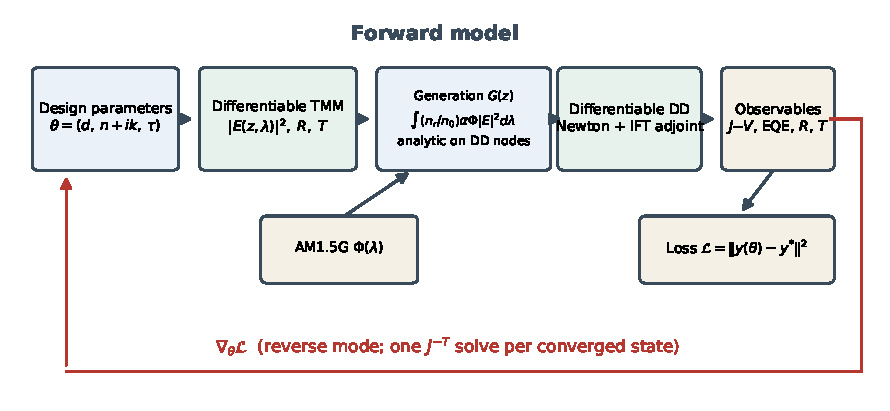
\includegraphics[width=\columnwidth]{figures/fig1_framework.pdf}
  \caption{UniDD forward model and reverse-mode gradient path. The generation
  rate is evaluated analytically on the drift--diffusion nodes; the backward
  pass requires one transposed Jacobian solve per converged state.}
  \label{fig:framework}
\end{figure}

\subsection{Numerical configuration}
\label{sec:config}

Table~\ref{tab:config} lists the reference configuration. The optical stack
is air / TiO$_2$ (50~nm, $\tilde n=2.0$) / absorber (480~nm,
$\tilde n=2.55+ik$) / spiro-OMeTAD (150~nm, $\tilde n=1.5+0.005i$) /
glass-equivalent substrate ($\tilde n=1.5$). The absorber extinction
coefficient is $k(\lambda)=k_{\mathrm{amp}}\exp[-\mathrm{ReLU}(\lambda-800)/60]+10^{-3}$
with $\lambda$ in nm and $k_{\mathrm{amp}}=0.72$, or a six-knot
piecewise-linear spectrum in the eight-parameter problem. The solar input is
a coarse tabulation of the ASTM G173 AM1.5G spectrum~\cite{astm2020} sampled
at 50~nm intervals from 300 to 1000~nm and linearly interpolated onto 41
equally spaced wavelengths from 350 to 800~nm; efficiencies are normalised
to the standard 100~mW\,cm$^{-2}$ incident power density. The DD device uses $T=300$~K, $E_g=1.55$~eV,
$\varepsilon_r=6.5$, $N_c=2.2\times10^{24}$~m$^{-3}$,
$N_v=1.8\times10^{25}$~m$^{-3}$, ideal selective contacts with
$n_L=2.2\times10^{24}$ and $p_R=1.8\times10^{25}$~m$^{-3}$,
$\mu_n=\mu_p=2\times10^{-4}$~m$^2$\,V$^{-1}$\,s$^{-1}$ and
$\tau_n=\tau_p=300$~ns. All computations use float64. The complete suite is
deterministic with seed 0 and requires about 25~min on one CPU core.

\begin{table}[t]
\caption{Reference configuration used in the core experiments E0--E4
and the supplements E4-H, E4-C and E5.}
\label{tab:config}
\centering
\small
\begin{tabular}{lll}
\toprule
Component & Parameter & Value \\
\midrule
Optics & stack & air / TiO$_2$ / absorber / HTL / substrate \\
       & layer thicknesses & 50 / 480 / 150 nm \\
       & absorber index & $2.55 + i\,k(\lambda)$ \\
       & wavelength grid & 41 points, 350--800 nm \\
       & incident spectrum & coarse AM1.5G (ASTM G173) \\
Device & nodes $N$ & 73 (production), 49--145 (convergence) \\
       & temperature & 300 K \\
       & band gap / $\varepsilon_r$ & 1.55 eV / 6.5 \\
       & mobility $\mu_{n,p}$ & $2\times10^{-4}$ m$^2$\,V$^{-1}$\,s$^{-1}$ \\
       & SRH lifetime $\tau_{n,p}$ & 300 ns \\
Solver & Newton tolerance & $10^{-9}\,qG_{\max}$, floor $3\times10^2$ A\,m$^{-3}$ \\
       & potential damping cap & 0.4 V \\
       & bias-continuation step & 0.05 V \\
       & adjoint system size & $3(N-2)=213$ \\
\bottomrule
\end{tabular}
\end{table}

%% ============================================================================
\section{Results and discussion}
\label{sec:results}
%% ============================================================================

\subsection{E0: external validation of the optical model}
\label{sec:e0}

We first test the optics against quantities that do not depend on the
electrical solver. Table~\ref{tab:validation} (upper block) summarises the
six checks, all of which pass. With layer-by-layer integration on a 2001-point
per-layer grid, $A_{\mathrm{field}}$ agrees with $1-R-T$ to
$1.44\times10^{-6}$; the deviation falls from $1.44\times10^{-4}$ at 201
points to $2.31\times10^{-5}$ at 501 points and to $1.44\times10^{-6}$ at
2001 points, consistent with the second-order convergence of the trapezoidal
rule (Fig.~\ref{fig:optics}a). A global integration grid that straddles
material interfaces does not converge monotonically, which is why the
integration is performed layer by layer.

The regression test has power: if the factor $n_r/n_0$ is omitted, the mean
absorptance drops from 0.9549 to 0.3745 and the maximum deviation from
$1-R-T$ rises to 0.592. For an index-matched absorbing slab the model
reproduces $A=1-\exp(-\alpha d)$ to $1.57\times10^{-8}$ with $R=0$ exactly.
Finally, the difference between coherent and incoherent absorption falls from
0.167 at 200~nm thickness to $4.20\times10^{-8}$ at 3000~nm
(Fig.~\ref{fig:optics}b), confirming that the coherent model degenerates to
the ray-optics limit for optically thick layers.

\begin{figure}[t]
  \centering
  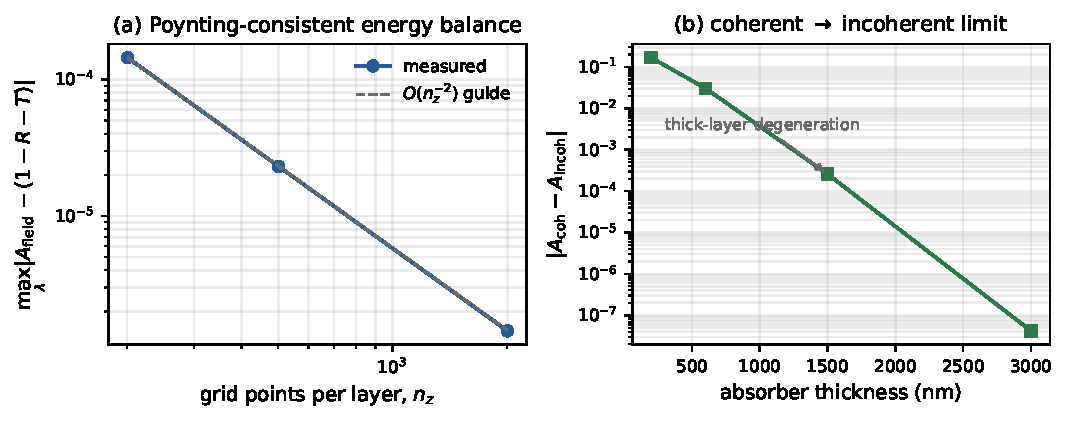
\includegraphics[width=\columnwidth]{figures/fig2_optical_validation.pdf}
  \caption{(a) Maximum deviation of the volume-integrated absorbed fraction
  from $1-R-T$ versus the number of integration points per layer; the dashed
  line is an $O(n_z^{-2})$ guide. (b) Degeneration of coherent absorption to
  the incoherent limit with increasing absorber thickness.}
  \label{fig:optics}
\end{figure}

\subsection{E1: gradient verification}
\label{sec:e1}

Gradient correctness is assessed at three levels (Table~\ref{tab:validation},
middle block). For the isolated TMM chain, AD and central finite differences
agree to $6.73\times10^{-11}$. For the isolated DD paths, the relative
deviation is $7.60\times10^{-6}$ (optical coupling) and
$4.40\times10^{-5}$ (electrical parameters). For the full composite chain,
per-parameter derivatives agree with fourth-order Richardson-extrapolated
central differences to $2.21\times10^{-4}$ ($d_{\mathrm{abs}}$),
$2.78\times10^{-3}$ ($k_{\mathrm{amp}}$) and $1.30\times10^{-4}$
($\log\tau$); the directional derivative agrees to $4.27\times10^{-4}$
(Fig.~\ref{fig:gradients}a).

The residual error is dominated by cancellation, not by the adjoint solve.
For the thickness derivative the optical contribution is
$-4.925\times10^{-3}$ and the electrical contribution
$+4.816\times10^{-3}$: two terms of comparable magnitude subtract to give
$-1.09\times10^{-4}$, a cancellation ratio of 45.05. The adjoint equation
itself is solved to a relative residual of $3.25\times10^{-14}$ with a
single iterative-refinement pass, and additional refinement passes do not
improve it. Consistently, sweeping the Newton residual floor over five orders
of magnitude leaves the full-chain deviation unchanged at
$4.27\times10^{-4}$ (Fig.~\ref{fig:gradients}b): the error is
finite-difference round-off amplified by cancellation, not solver
tolerance. The solver walk reaches residuals of 20.5, 614,
$1.50\times10^{4}$ and $6.52\times10^{4}$~A\,m$^{-3}$ at 0, 0.3, 0.6 and
0.9~V in 23, 15, 17 and 17 iterations, all converged on the physical scale
$qG_{\max}$.

This last point is worth emphasising because it changed the outcome of the
study. In an earlier version of the solver, convergence was declared
relative to the warm-start residual; after a bias step that residual can be
$10^{17}$~A\,m$^{-3}$, so the returned iterate had $|F|\sim10^{8}$ and was
not a root. IFT gradients evaluated there were biased by about 1.5\% and did
not improve when tolerances were tightened. Convergence on the physical
scale with a Newton-step test (Eq.~\eqref{eq:convergence}) removed the bias.

\begin{figure}[t]
  \centering
  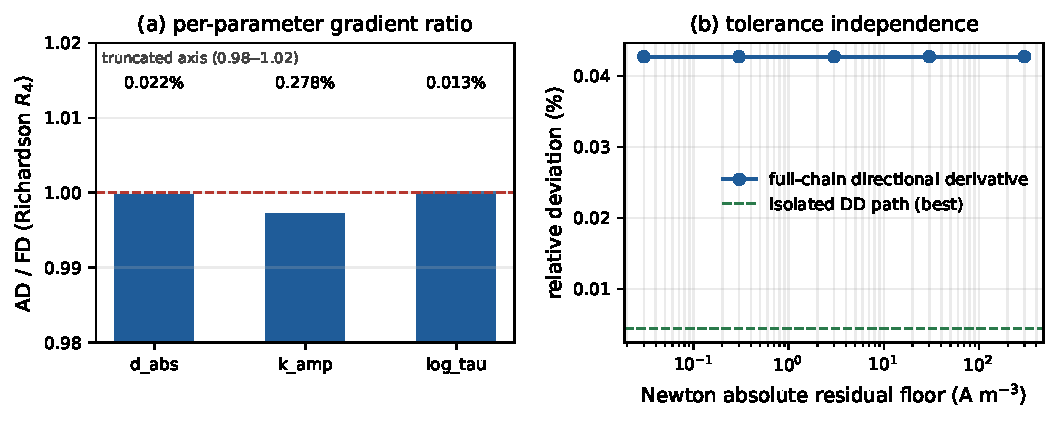
\includegraphics[width=\columnwidth]{figures/fig4_gradients.pdf}
  \caption{(a) Ratio of automatic derivatives to fourth-order Richardson
  finite differences for each design parameter; labels give the relative
  deviation and the vertical axis is explicitly truncated and labelled
  in the panel. (b) Relative deviation of the full-chain directional derivative
  as the Newton residual floor is swept, compared with the best isolated DD
  path.}
  \label{fig:gradients}
\end{figure}

\subsection{E2: physical validation and reference-device figures of merit}
\label{sec:e2}

Six of seven pre-specified physical checks pass; the failing one is the
coarsest-grid mesh test, reported together with its Richardson
extrapolation (Table~\ref{tab:validation}, lower block). At thermal equilibrium the dark
current is exactly zero to float64; the dark $J$--$V$ has an ideality factor
of 1.208, within the expected 1--2 range. For spatially uniform generation
the computed $J_{\mathrm{sc}}=35.42$~mA\,cm$^{-2}$ reaches 0.980 of the
analytic limit $qGL=36.15$~mA\,cm$^{-2}$. The EQE-integrated short-circuit
current, 29.68~mA\,cm$^{-2}$, differs from the $J$--$V$ value
29.95~mA\,cm$^{-2}$ by 0.89\%; the mean EQE over 21 wavelengths from 380 to
790~nm is 0.881. The optical upper bound on $J_{\mathrm{sc}}$ obtained by
assuming that every absorbed photon is collected is 32.47~mA\,cm$^{-2}$, so
the DD result (29.95) is consistent with, and 7.8\% below, that bound.
$R+T\le1$ holds at every wavelength, with mean $R=0.0436$ and mean
$T=0.0010$.

For the reference stack the illuminated $J$--$V$
(Fig.~\ref{fig:device}a) gives $J_{\mathrm{sc}}=29.95$~mA\,cm$^{-2}$,
$V_{\mathrm{oc}}=1.110$~V, $\mathrm{FF}=0.835$ and
$\eta=27.74\%$, with the maximum-power point at 1.00~V and
27.74~mA\,cm$^{-2}$. These numbers must be read as \emph{synthetic}
illustrations: the incident spectrum is a coarse 350--800~nm tabulation,
radiative and Auger recombination, surface recombination, series resistance
and a band-gap cutoff are absent, and the efficiency is normalised to the
conventional 100~mW\,cm$^{-2}$ irradiance. They are not a device-efficiency
prediction and are far from constituting a claim against detailed-balance
limits~\cite{shockley1961, richter2013}.

The one check that does not pass as originally formulated is the mesh
criterion, which required the short-circuit current at $N=49$ and $N=97$ to
agree within 2\%; the measured change is 2.48\%. We therefore extended the
study to $N=145$ (Fig.~\ref{fig:device}b). $J_{\mathrm{sc}}$ increases
monotonically as 29.417, 29.950, 30.164, 30.268 and 30.324~mA\,cm$^{-2}$
for $N=49,73,97,121,145$; the observed order is 2.72 and Richardson
extrapolation gives 30.412~mA\,cm$^{-2}$. The production grid ($N=73$)
therefore carries a 1.52\% discretisation uncertainty, while the change from
$N=73$ to the next refinement ($N=97$) is only 0.71\%. The original failure
is attributable to an under-resolved \emph{coarsest} grid rather than to an
inconsistent discretisation, and we report the uncertainty explicitly.

\begin{figure}[t]
  \centering
  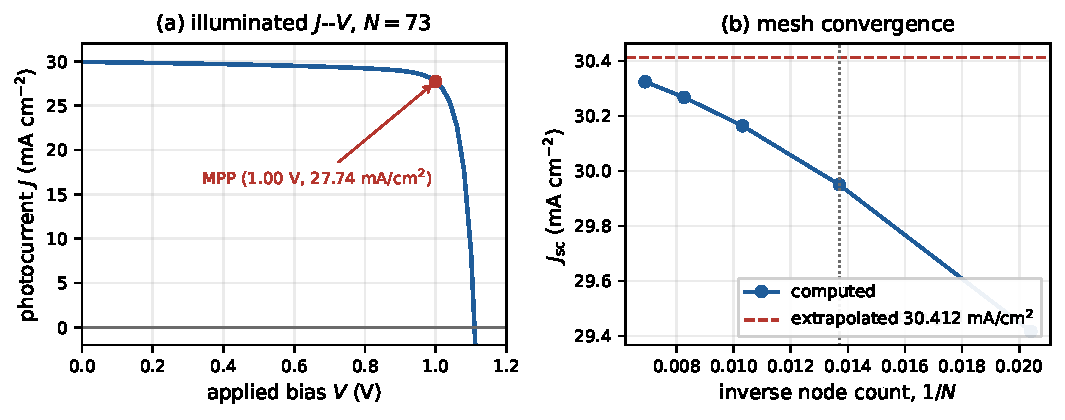
\includegraphics[width=\columnwidth]{figures/fig3_device_and_mesh.pdf}
  \caption{(a) Illuminated $J$--$V$ characteristic of the reference stack on
  the production grid and its maximum-power point. (b) Mesh convergence of
  $J_{\mathrm{sc}}$; the dashed line is the Richardson-extrapolated limit and
  the dotted line marks the production grid.}
  \label{fig:device}
\end{figure}

\begin{table}[t]
\caption{Validation summary. E0: external optical checks; E1: gradient
checks; E2: physical checks. ``Pass'' refers to the pre-specified criteria.}
\label{tab:validation}
\centering
\small
\begin{tabular}{llcc}
\toprule
Test & Observed value & Criterion & Pass \\
\midrule
\multicolumn{4}{l}{\emph{E0 --- optics (6/6 pass)}}\\
$A_{\mathrm{field}}$ vs.\ $1-R-T$, 2001 pts & $1.44\times10^{-6}$ & $<10^{-4}$ & yes \\
grid convergence of the above & $1.44\!\times\!10^{-4}\to1.44\!\times\!10^{-6}$ & monotone & yes \\
regression power without $n_r/n_0$ & max dev.\ 0.592 & $>0.1$ & yes \\
Beer--Lambert, index-matched slab & $1.57\times10^{-8}$ & $<10^{-6}$ & yes \\
index-matched reflection & 0 & $<10^{-10}$ & yes \\
coherent $\to$ incoherent, 3000~nm & $4.20\times10^{-8}$ & $<10^{-6}$ & yes \\
\midrule
\multicolumn{4}{l}{\emph{E1 --- gradients (pass)}}\\
pure TMM chain, AD vs.\ FD & $6.73\times10^{-11}$ & $<10^{-6}$ & yes \\
isolated DD optical path & $7.60\times10^{-6}$ & $<10^{-3}$ & yes \\
isolated DD electrical path & $4.40\times10^{-5}$ & $<10^{-3}$ & yes \\
full chain, worst per parameter & $2.78\times10^{-3}$ & $<10^{-2}$ & yes \\
full chain, directional & $4.27\times10^{-4}$ & $<10^{-2}$ & yes \\
adjoint relative residual & $3.25\times10^{-14}$ & $<10^{-9}$ & yes \\
\midrule
\multicolumn{4}{l}{\emph{E2 --- physics (6/7 pass)}}\\
$R+T\le1$ at every $\lambda$ & yes & yes & yes \\
equilibrium dark current & 0~A\,m$^{-2}$ & $<10^{-6}$ & yes \\
dark ideality factor & 1.208 & 1--2 & yes \\
uniform-$G$ $J_{\mathrm{sc}}/qGL$ & 0.980 & $\pm5\%$ & yes \\
EQE vs.\ $J$--$V$ $J_{\mathrm{sc}}$ & 0.89\% & $<5\%$ & yes \\
$J_{\mathrm{sc}}\le 1.02\times$ optical bound & 29.95 vs.\ 32.47 & yes & yes \\
$N=49$ vs.\ $N=97$ $J_{\mathrm{sc}}$ change & 2.48\% & $<2\%$ & \textbf{no} \\
\bottomrule
\end{tabular}
\end{table}

\subsection{E3: three-parameter inverse design}
\label{sec:e3}

The synthetic target is
$(d^{*},k^{*},\tau^{*})=(480~\mathrm{nm},\,0.72,\,300~\mathrm{ns})$; the
starting point is $(300~\mathrm{nm},\,0.35,\,1.5~\mu\mathrm{s})$. With the
full observable set of Eq.~\eqref{eq:observables}, L-BFGS driven by exact IFT
gradients reduces the loss from $6.45\times10^{-3}$ to
$3.32\times10^{-13}$ in 44 function/gradient evaluations (106~s). The
recovered values are $d=479.990$~nm, $k=0.720015$ and
$\tau=3.0000\times10^{-7}$~s, i.e.\ relative errors of
$2.02\times10^{-5}$, $2.12\times10^{-5}$ and
$3.93\times10^{-7}$ in $\log\tau$ (Table~\ref{tab:inverse}). All three
parameters are recovered to within 0.0022\%.

This result depends on the inclusion of $R(\lambda)$ and $T(\lambda)$. With
$J$--$V$ and EQE alone, a thinner and more strongly absorbing layer produces
nearly indistinguishable electrical observables, and the $(d,k)$ pair is
only weakly identifiable. Reflectometry and transmission measurements are
routine and, because they are computed directly by the TMM recursion, they
add no DD solves. The identifiability analysis is itself a useful output of
having exact gradients.

\begin{table}[t]
\caption{Three-parameter inverse design (E3).}
\label{tab:inverse}
\centering
\small
\begin{tabular}{llll}
\toprule
Parameter & Target & Recovered & Relative error \\
\midrule
$d$ (nm) & 480.0 & 479.990 & $2.02\times10^{-5}$ \\
$k_{\mathrm{amp}}$ & 0.72 & 0.720015 & $2.12\times10^{-5}$ \\
$\tau$ (s) & $3.0000\times10^{-7}$ & $2.999999\times10^{-7}$ & $3.93\times10^{-7}$ in $\log\tau$ \\
\midrule
final loss & \multicolumn{3}{l}{$3.32\times10^{-13}$ after 44 evaluations (106~s)} \\
\bottomrule
\end{tabular}
\end{table}

\subsection{E4: evaluation-count benchmark}
\label{sec:e4}

The derivative-free baseline is counted in true function calls. A Nelder--Mead
\emph{iteration} is not a function evaluation: a shrink step costs $n+1$
objective calls. Earlier results in this project recorded one history entry
per iteration and were therefore optimistic about the baseline by a large
factor. The benchmark reported here records the cumulative number of
$f()$ calls after every call (Fig.~\ref{fig:optimization}).

In the three-dimensional problem, L-BFGS reaches a loss of $10^{-3}$ in 7
calls and $10^{-4}$ in 16, whereas Nelder--Mead reaches $10^{-3}$ in 7 calls
but never reaches $10^{-4}$ within 150 calls (best
$1.23\times10^{-4}$). At the common budget of 49 calls the losses are
$9.53\times10^{-15}$ and $1.25\times10^{-4}$. Because the derivative-free
run is censored, the call-count advantage at $10^{-4}$ is at least
$150/16=9.4\times$, at $10^{-5}$ at least $7.9\times$, and at $10^{-6}$ at
least $7.5\times$.

In the eight-dimensional problem (thickness, lifetime and six spectral
knots), L-BFGS reaches $10^{-3}$ in 7 calls against 21 for Nelder--Mead, a
$3.0\times$ advantage, and at the common budget of 44 calls attains
$1.85\times10^{-4}$ against $6.35\times10^{-4}$. Neither method reaches
$10^{-4}$: L-BFGS stalls at $1.85\times10^{-4}$ after 44 calls and
Nelder--Mead at $2.24\times10^{-4}$ after 300 calls. The recovered thickness
is 394.9~nm against a target of 460~nm (14.2\% error) and the six spectral
knots are poorly recovered. The pre-specified target of a $\ge10\times$
evaluation reduction in eight dimensions is therefore \textbf{not met}, and
we do not claim it. The measured forward-plus-adjoint cost is a factor of 1.10 over a
single forward solve (forward 2.21~s, forward+backward 2.43~s in the 3-D
case), not the 1.05 quoted in earlier internal notes.

Table~\ref{tab:benchmark} gives the exact counts. The conclusion is
that exact IFT gradients give a clear advantage for tight tolerances in low
dimension and a modest (about $3\times$) advantage at moderate accuracy in
eight dimensions, at a 10\% cost per evaluation. The eight-dimensional
problem also exposes weak identifiability of a spectrally resolved extinction
coefficient from the present observable set; more informative observables or
regularisation would be needed before claiming practical high-dimensional
reconstruction.

\begin{figure}[t]
  \centering
  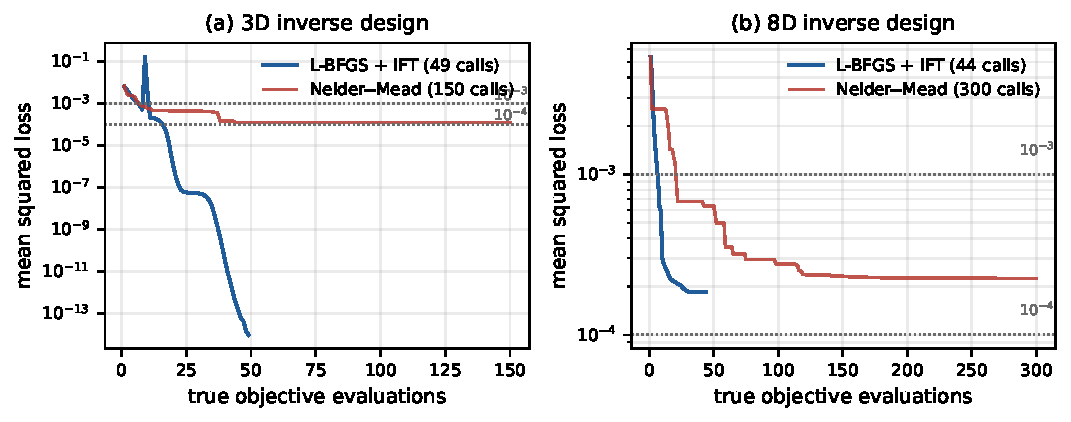
\includegraphics[width=\columnwidth]{figures/fig5_optimization.pdf}
  \caption{Mean squared loss versus the true number of objective evaluations
  for (a) the three-parameter and (b) the eight-parameter inverse problems.
  Dotted lines mark losses of $10^{-3}$ and $10^{-4}$.}
  \label{fig:optimization}
\end{figure}

\begin{table}[t]
\caption{Evaluation-count benchmark (E4). ``n.r.'' = not reached within the
stated budget.}
\label{tab:benchmark}
\centering
\small
\begin{tabular}{lcc}
\toprule
Quantity & 3-D & 8-D \\
\midrule
budget (L-BFGS / NM), calls & 49 / 150 & 44 / 300 \\
final loss, L-BFGS & $9.53\times10^{-15}$ & $1.85\times10^{-4}$ \\
final loss, NM & $1.23\times10^{-4}$ & $2.24\times10^{-4}$ \\
calls to $10^{-3}$ (L-BFGS / NM) & 7 / 7 & 7 / 21 \\
calls to $10^{-4}$ (L-BFGS / NM) & 16 / n.r. & n.r. / n.r. \\
loss at common budget, L-BFGS & $9.53\times10^{-15}$ & $1.85\times10^{-4}$ \\
loss at common budget, NM & $1.25\times10^{-4}$ & $6.35\times10^{-4}$ \\
forward-plus-adjoint cost factor & 1.10 & 1.10 \\
$\ge10\times$ criterion & not met & \textbf{not met} \\
\bottomrule
\end{tabular}
\end{table}

\subsection{A pre-specified high-dimensional supplement (E4-H)}
\label{sec:e4h}

The verdict of Section~\ref{sec:e4} is unchanged: with the original protocol
the $\ge10\times$ target is \textbf{not met} in three or eight dimensions.
That section also identifies two obstacles to high-dimensional inversion,
namely weak identifiability of a spectrally resolved extinction coefficient
from the available observables and the non-differentiable piecewise-linear
spectrum used at the wavelength knots. We therefore ran a separate supplement
whose protocol was fixed before execution and recorded in the accompanying
result file, to test whether exact gradients become decisive when the design
space is enlarged and the inverse problem is made better posed. The design
space has 16 parameters (thickness, 14 smooth Gaussian radial-basis spectral
coefficients and lifetime), the $R/T$ observables are sampled at 16
wavelengths, and both optimisers start from the same point. The loss, the
threshold ladder, the optimiser settings and the per-call bookkeeping are
those of Section~\ref{sec:e4}; the budgets were increased for both methods,
to 200 calls for L-BFGS and 600 for Nelder--Mead.

L-BFGS with exact IFT gradients reached $10^{-4}$ in 23 calls, $10^{-5}$ in
34 and $10^{-6}$ in 45, ending at $1.40\times10^{-7}$ after 65 calls.
Nelder--Mead did not reach $10^{-4}$ within its 600 calls (best
$1.19\times10^{-4}$); at the common budget of 65 calls its best loss was
$7.75\times10^{-4}$. Under the same censoring rule as in E4 these counts give
lower bounds of $26.1\times$, $17.6\times$ and $13.3\times$ at the three
tight thresholds, so the $\ge10\times$ criterion is met in this supplementary
setting. These are bounds rather than measured ratios: at the loosest
informative threshold, $10^{-3}$, both methods succeeded and the measured
advantage was $8.57\times$ (7 against 60 calls). The derivative-free run was
censored only marginally above $10^{-4}$, and a forward-plus-adjoint evaluation cost 1.22
times a forward solve.

This supplement does not revise E4. Dimension, spectral parametrisation and
the number of $R/T$ observables were changed together, so the result does not
isolate dimension as the cause of the improvement; all targets remain
synthetic inverse crimes. A controlled study varying one factor at a time,
with multiple starting points and measurement noise, is still needed before
a general efficiency claim can be made.

\subsection{Controlled-dimension and robustness supplements (E4-C, E5)}
\label{sec:supplements}

The E4-H supplement changed the design dimension, the spectral
parametrisation and the number of $R/T$ observables at the same time, so its
censored PASS could not be attributed to dimension alone. E4-C removes that
ambiguity. Both arms use the same RBF basis and width, the same true spectrum,
the same start point, the same 44 normalised observables, the same loss, the
same optimiser settings and the same evaluation budgets; the only factor that
differs is the number of free design variables. The 8-D spectral coefficients
are mapped into the 14-dimensional RBF coefficient space by a fixed
row-normalised Gaussian matrix, so the 8-D arm is an exact linear subspace of
the 16-D arm rather than a differently parametrised problem. The two synthetic
targets agree to $|\Delta y|_{\max} = 0$,
and a constant coefficient vector maps to itself to $1.1\times10^{-16}$.
The experiment is deliberately noise-free, because its purpose is to isolate
one factor; noise and multiple starts are handled separately in E5.
Table~\ref{tab:e4c} reports the evaluation counts.

\begin{table}[t]
\centering
\footnotesize
\caption{E4-C evaluation counts to reach a target loss. Each cell gives the
Nelder--Mead count (numerator) over the L-BFGS count (denominator), so the
quoted ratio is the evaluation-count advantage of the gradient-based method.
Entries marked $\ge$ are censored lower bounds, not measured ratios: the
derivative-free run stopped at its budget before reaching that loss.}
\label{tab:e4c}
\begin{tabular}{lp{5.0cm}p{5.0cm}}
\toprule
Target loss & 8-D & 16-D \\
\midrule
0.01 & 1/1 = 1.00$\times$ (measured) & 1/1 = 1.00$\times$ (measured) \\
$10^{-3}$ & 25/7 = 3.57$\times$ (measured) & 60/7 = 8.57$\times$ (measured) \\
$10^{-4}$ & $\ge$301/25 = $\ge$12.04$\times$ (censored) & $\ge$300/23 = $\ge$13.04$\times$ (censored) \\
$10^{-5}$ & not reached & $\ge$300/33 = $\ge$9.09$\times$ (censored) \\
$10^{-6}$ & not reached & $\ge$300/43 = $\ge$6.98$\times$ (censored) \\
\bottomrule
\end{tabular}
\end{table}

L-BFGS used 67 (8-D) and 64 (16-D)
forward/adjoint evaluations, and Nelder--Mead used 301 and 300
function calls, reaching best losses of $3.0\times10^{-4}$ and $2.2\times10^{-4}$.
Of the 10 arm--threshold combinations, 4
yield a measured ratio (2 of which are the trivial
first-call row at the loosest threshold), 4 are censored,
and the remaining 2 (both in the 8-D arm) reached the
target loss with neither optimiser (``not reached''). The four censored
entries comprise the $10^{-4}$ row of both arms and the two stricter
thresholds of the 16-D arm.
Measured, uncensored comparisons are available at 1 informative threshold: at $10^{-3}$ the measured advantage is 3.57$\times$ (8-D) against 8.57$\times$ (16-D). The 16-D advantage is larger at every such threshold, consistent with a dimension effect under this fixed-observation protocol. At $10^{-3}$ L-BFGS used 7 and 7 calls in the two arms, whereas Nelder--Mead used 25 and 60. The ratio grows because the derivative-free simplex needs more calls as the dimension increases, while the gradient-based count is unchanged. Because the 8-D arm is a subspace of the 16-D one, the higher-dimensional problem is less constrained, which also lowers its final loss ($1.5\times10^{-7}$ versus $2.7\times10^{-5}$). This is a single-start, noise-free, single-model result, not a general efficiency claim. At $10^{-4}$ and stricter losses the derivative-free run is censored in both arms, so the recorded 12.04$\times$ (8-D) and 13.04$\times$ (16-D) are lower bounds rather than measured ratios; the E4-H PASS at that threshold therefore remains a censored result.

E5 addresses a different question: whether the picture survives changes of
start point, observation noise and the choice of derivative-free comparator.
Two deterministically perturbed starts were run against 5
baselines (Nelder--Mead, Powell, differential evolution, dual annealing and an
in-house RBF--UCB surrogate), each with a budget of 80 true
function calls and 1\% relative Gaussian observation noise. At the
common budget the smallest mean best loss was 6.540e-04 (Powell) and the largest was 1.001e-03 (DualAnnealing);
7 of 10 runs reached $10^{-3}$ and 0 of 10
reached $10^{-4}$. Because the noisy objective has a loss floor, E5 is used as
robustness evidence only; no speedup is claimed from it. The RBF--UCB baseline
is a lightweight in-house implementation, not a tuned Bayesian-optimisation
library.

Neither supplement changes the main verdict: the $\ge10\times$ target is
\textbf{not met} in eight dimensions, and the E4-H PASS remains a censored
lower bound. All targets are synthetic inverse crimes; an independent
SCAPS-1D comparison is reported in Section~\ref{sec:scaps}, and no
experimental calibration has been performed.

\subsection{Scope of the coherent optical model}
\label{sec:ablation}

Retaining the interference term is a modelling choice rather than a universal
accuracy requirement. To locate its practical scope, the reference device and
a grid of five absorption strengths ($k$ amplitude $0.02$--$0.72$) and three
absorber thicknesses ($120$, $240$, $480$~nm) were recomputed with the
coherent field replaced by a single-pass Beer--Lambert profile that keeps the
same Fresnel transmission amplitude. At the reference $480$~nm device the
short-circuit current changes by only $0.0071\%$ ($29.9499$ against
$29.9477$~mA\,cm$^{-2}$) and the thickness gradient by $1.91\%$; the coherent
generation profile has one interior extremum where the single-pass profile is
monotone. Over the $15$ grid points the largest $J_{\mathrm{sc}}$ difference
is $4.87\%$, whereas the largest thickness-gradient difference is $39.85\%$
at $120$~nm and $k=0.72$. Coherent optics therefore matters chiefly for
derivatives and inverse design in thin, strongly absorbing stacks, and much
less for predicting $J_{\mathrm{sc}}$ in the reference device. We do not
claim that a coherent optical model is necessary in general. The ablation and
its recorded output are distributed with the code
(\texttt{experiments\_optics\_ablation.py},
\texttt{results\_optics\_ablation.json}).

\section{Limited cross-code sanity check with SCAPS-1D 3.3.12}
\label{sec:scaps}

The electrical kernel was compared with SCAPS-1D 3.3.12~\cite{burgelman2000}
using the script chain distributed with the code. Because UniDD solves the
drift--diffusion equations on the absorber only, with the transport layers
entering the optics and the contact boundary values, the SCAPS device was
built as a single absorber layer with selective surface-recombination
contacts. The coherent UniDD generation profile was imported in SI units
(m$^{-3}$\,s$^{-1}$) and the native SCAPS $J$--$V$, QE and generation curves
were exported through the SCAPS script interface, together with
SCAPS-generated graphs and the solver diagnostic log. The four acceptance
criteria were fixed before execution and were not revised afterwards.

\begin{table}[t]
\caption{Pre-specified acceptance criteria, reproduced verbatim from the
distributed protocol, and the outcome of the SCAPS-1D 3.3.12 comparison.
Errors are evaluated on the common converged voltage or wavelength range;
dark-current RMSE is in mA\,cm$^{-2}$.}
\label{tab:scaps}
\centering
\footnotesize
\begin{tabular}{lp{4.3cm}p{4.0cm}c}
\toprule
Quantity & Criterion & Measured & Verdict \\
\midrule
Dark $J$--$V$ & RMSE $<0.05$ \emph{or} mean rel.\ $<5\%$ & RMSE $1.44\times10^{-3}$; mean rel.\ 212.10\% & PASS \\
Illuminated $J$--$V$ & $J_{\mathrm{sc}}<5\%$, $V_{\mathrm{oc}}<20$~mV, FF $<5\%$ & $J_{\mathrm{sc}}$ 7.03\%; $V_{\mathrm{oc}}$, FF n/a & FAIL \\
EQE & RMSE $<0.05$ & 0.096 & FAIL \\
$G(z)$ read-back & RMSE/$\overline{G}<2\%$ & $2.4\times10^{-4}\%$ & PASS \\
\bottomrule
\end{tabular}
\end{table}

\textbf{Comparability, fixed before the run.} The dark $J$--$V$ and the
generation read-back are comparable by construction: the former has no
generation term, and the latter is a direct unit-conversion and mesh
interpolation check of the imported profile. The illuminated $J$--$V$ and the
EQE are \emph{not comparable by construction}: UniDD imposes Dirichlet
carrier densities at the contacts, whereas SCAPS uses flat-band,
surface-recombination contacts, and SCAPS recomputes its QE from its own
internal wavelength-resolved absorption while UniDD imports a
wavelength-integrated $G(z)$. Their FAIL verdicts are retained verbatim as
pre-specified outcomes and are reported as model-mismatch diagnostics, not
as a failure rate of the drift--diffusion kernel. No criterion, threshold
or verdict was added, removed or relaxed after the data were produced.

Two of the four pre-specified criteria pass (Table~\ref{tab:scaps}); the
remaining two are the non-comparable ones. The dark-current criterion has two
branches because the UniDD dark current is essentially zero: a mean relative
error of 212.10\% is not informative there, so the absolute-RMSE branch
decides that verdict. Over the common converged range
$0$--$0.8$~V the dark curves agree to
$1.44\times10^{-3}$~mA\,cm$^{-2}$ RMSE; SCAPS stops the dark sweep at
$0.82$~V. The SCAPS read-back of the imported $G(z)$ deviates from the
UniDD profile by $2.4\times10^{-4}\%$ of the mean generation rate, which
checks the unit conversion and the interpolation onto the SCAPS mesh. The
short-circuit currents differ by 7.03\% ($32.06$ against
$29.95$~mA\,cm$^{-2}$), and the EQE shape check gives an RMSE of $0.096$.
Open-circuit voltage and fill factor cannot be defined for the SCAPS curve:
with flat-band, surface-recombination contacts and an intrinsic absorber the
illuminated SCAPS $J$--$V$ is almost independent of bias up to the
convergence cut at $1.06$~V, whereas UniDD imposes Dirichlet carrier
densities at the contacts. This is a model mismatch rather than a
discretisation error. The comparison is therefore reported as a limited
cross-code sanity check; it does not constitute a validation of UniDD
against SCAPS-1D, and no experimental calibration has been performed. The
SCAPS binary is closed source and is not redistributed for licensing
reasons; the single-layer definition, the imported generation profile, the
script chain, the native SCAPS outputs and the solver diagnostic log are
shipped together with \texttt{scaps\_version.txt}, which pins the executable
version and build date and the SHA-256 of the LabWindows/CVI run-time
deployment. This pinned archive allows the comparison to be audited without
re-running SCAPS-1D.

\section{Model choice and gradient cost}
\label{sec:evidence}

The ablation of Section~\ref{sec:ablation} identifies where coherent optics
changes derivatives but not whether it changes a design decision. This
section supplies that missing evidence and quantifies the cost of the
adjoint against the finite-difference baseline that was previously absent.
All three experiments are synthetic; none is an experimental validation.

\subsection{Optical-model misspecification in inverse design}
\label{sec:evidence-inverse}

A thin, strongly absorbing stack ($d=120$~nm, $k=0.72$, $\tau=3\times10^{-7}$~s)
was chosen at the grid point where the recorded regime scan reports the
largest thickness-gradient contrast. Twelve normalised observations (six
$J$--$V$ points and six EQE points) were generated with the coherent model.
The inverse variable is the absorber thickness alone, with $k$ and $\tau$
fixed at their true values: a preliminary three-parameter version stalled in
local minima on both arms, reflecting the weak identifiability already
reported in E4, and would have confounded the model-choice question. The
loss was therefore scanned on a deterministic grid (80--300~nm in 5~nm steps
plus a 1~nm local refinement) rather than trusted to a local optimiser. Two
arms used the same grid and budget, changing only the optical generation
model inside the inverse loop: a correctly specified coherent arm and a
misspecified single-pass arm that keeps the same Fresnel amplitude,
$\alpha(\lambda)$, AM1.5G flux and $n_r/n_0$ factor. Reflection/transmission
observations were excluded so that each arm is a self-consistent forward
model. The target is generated by the same forward model as the control arm,
so this is a synthetic inverse crime; what it measures is
\emph{model-misspecification bias}, not identifiability from measured data.

\begin{table}[t]
\caption{One-parameter thickness inversion under a correctly specified and a
misspecified optical model. Truth: $d=120$~nm, $k=0.72$,
$\tau=3\times10^{-7}$~s.}
\label{tab:optical_inverse}
\centering
\footnotesize
\begin{tabular}{lcc}
\toprule
Quantity & Coherent TMM & Single-pass \\
\midrule
Best-fit $d$ (nm) & 120.00 & 121.00 \\
Loss at best fit & 0.00e+00 & 2.28e-04 \\
$\dd L/\dd d$ at 200~nm & 1.500e-04 & 1.874e-04 \\
Forward evaluations & 54 & 54 \\
\bottomrule
\end{tabular}
\end{table}

The control recovers the generating thickness, whereas the single-pass arm
prefers a thickness biased by 0.83\% (Table~\ref{tab:optical_inverse}):
the two optical models rank designs differently. At a common starting
thickness their loss gradients differ by a factor of 1.25. Evaluated
with the coherent truth model, the misspecified solution leaves a normalised
observable RMSE of 2.310e-03, while its $J_{\mathrm{sc}}$ is
0.27\% above the coherent design: at this operating point the parameter bias
does not translate into a current penalty. Together with the $0.0071\%$
reference-current change reported in Section~\ref{sec:ablation}, this bounds
the claim. Coherent optics is material to parameter recovery and gradient
fidelity in thin, strongly absorbing stacks; it is not shown to be necessary
for $J_{\mathrm{sc}}$ prediction. This is a model-choice result from a
synthetic inverse crime, not a claim that coherent optics is generally
necessary and not an experimental validation. The experiment and its recorded
loss curves are distributed as \texttt{experiments\_optical\_inverse.py} and
\texttt{results\_optical\_inverse.json}.

\subsection{Measured cost of the dense adjoint}
\label{sec:evidence-scaling}

Table~\ref{tab:adjoint_scaling} times a single-bias forward solve and a
forward-plus-adjoint evaluation on the five DD meshes used in the recorded
convergence study, together with the isolated dense
\texttt{torch.linalg.solve} of size $3(N-2)$ that the IFT node performs.
The isolated linear-algebra cost grows approximately as
$N^{1.85}$ over the measured range, while the end-to-end gradient
cost is dominated by the Newton iteration at these mesh sizes. The dense
adjoint is therefore adequate at the production grid $N=73$ but is the
limiting factor for much larger meshes; a sparse or matrix-free adjoint is
left as future work.

\begin{table}[t]
\caption{Measured adjoint cost versus DD mesh size. Best of repeated runs on
one CPU core; the last column times the isolated dense solve of size
$3(N-2)$.}
\label{tab:adjoint_scaling}
\centering
\footnotesize
\begin{tabular}{lccccc}
\toprule
$N$ & $3(N-2)$ & Forward (s) & Fwd\,+\,adj.\ (s) & Ratio & Dense solve (ms) \\
\midrule
49 & 141 & 0.174 & 0.240 & 1.38 & 0.08 \\
73 & 213 & 0.210 & 0.283 & 1.35 & 0.23 \\
97 & 285 & 0.255 & 0.326 & 1.28 & 0.34 \\
121 & 357 & 0.379 & 0.461 & 1.22 & 0.50 \\
145 & 429 & 0.405 & 0.521 & 1.28 & 0.64 \\
\bottomrule
\end{tabular}
\end{table}

\subsection{Finite-difference gradients with the same optimiser}
\label{sec:evidence-cost}

The derivative-free baselines of E4 and E5 do not isolate the value of the
adjoint, because they also change the optimiser. An additional arm therefore
reruns the recorded three-dimensional E4 case with central finite differences
($h=10^{-4}$) driving the same L-BFGS settings. At the common start point
the finite-difference and IFT gradients agree to cosine 1.00000. A
central-difference gradient costs 7 forward solves against
$1.10$ for a forward-plus-adjoint evaluation, a per-gradient ratio of
6.37. Counting every forward solve, including line-search
evaluations, the finite-difference arm needs 49 forward solves to
reach a loss of $10^{-3}$ against 7.69 forward-solve equivalents for
the IFT arm, a 6.37-fold advantage. This quantifies the net benefit
of the 10\% adjoint overhead. It is a three-dimensional cost comparison; it
does not revise the pre-specified eight-dimensional E4 verdict, and it is
not an experimental result. The arm and its recorded output are distributed
as \texttt{experiments\_fd\_baseline.py} and
\texttt{results\_fd\_baseline.json}; the scaling measurement is
\texttt{experiments\_adjoint\_scaling.py} with
\texttt{results\_adjoint\_scaling.json}.


%% ============================================================================
\section{Limitations and scope}
\label{sec:limitations}
%% ============================================================================

The present study is a methods paper and has four classes of limitation.

\textbf{Synthetic validation.} All targets are generated by the same forward
model, so the inverse-design experiments are inverse crimes: they establish
that the gradients are correct and that the optimisation machinery works, but
they do not establish identifiability from measured data. No comparison with
experimental $J$--$V$, EQE or ellipsometry data has been performed. An
independent comparison with SCAPS-1D 3.3.12 was carried out
(Section~\ref{sec:scaps}), but it is a limited cross-code sanity
check: two of four pre-specified criteria pass, and the illuminated
$J$--$V$ curves are not comparable because the contact models differ. Section~\ref{sec:scaps} documents the executed comparison and its
pre-specified criteria; experimental calibration remains the most
important next step before the framework can be used for device design.
A minimal programme is (i) spectroscopic ellipsometry for layer
thicknesses and $n(\lambda)+ik(\lambda)$, (ii) absolute EQE and dark
and illuminated $J$--$V$ on the same devices, and (iii) a
calibration/hold-out split over thicknesses and fabrication batches.

\textbf{Physical model.} The device model is one-dimensional, isothermal and
steady-state, with ideal selective ohmic contacts, Boltzmann statistics,
equal electron and hole mobilities, a single SRH lifetime and no radiative or
Auger recombination, no surface or grain-boundary recombination, no ionic
migration, no series/shunt resistance and no explicit band-gap cutoff in the
absorption spectrum. The solar input is a coarse 50-nm-sampled AM1.5G table
interpolated onto a 41-point grid spanning 350--800~nm. Consequently the
absolute figures of merit in
Section~\ref{sec:e2} are illustrative; they should not be compared with
measured efficiencies or with detailed-balance limits. The ablation of
Section~\ref{sec:ablation} further delimits the interference term: for
the reference device it changes $J_{\mathrm{sc}}$ by $0.0071\%$ only,
so coherent optics is not a generally necessary correction to the
current.

\textbf{Numerics.} The adjoint is formed by a dense $3(N-2)$ solve, which is
adequate at $N=73$ but scales cubically. Extensions to two-dimensional
devices would require sparse or matrix-free adjoint solves. The production
grid carries a 1.52\% uncertainty in $J_{\mathrm{sc}}$ relative to the
Richardson-extrapolated value. The full-chain thickness gradient suffers a
cancellation ratio of 45 between optical and electrical contributions, which
makes it sensitive to finite-difference round-off even though the adjoint
itself is solved to $10^{-14}$.

\textbf{Benchmark scope.} The $\ge10\times$ evaluation-count target is not
met in eight dimensions; the main E4 benchmark compares a single starting point,
a single noise-free synthetic target and two optimisers. The E4-C and E5 supplements of Section~\ref{sec:supplements} add a one-factor dimension control, multiple starts, measurement noise and five derivative-free baselines. They are robustness evidence and do not revise the $\ge10\times$ verdict stated above.

%% ============================================================================
\section{Conclusions}
\label{sec:conclusions}
%% ============================================================================

We have shown that a fully coupled drift--diffusion solver can be made
exactly differentiable at a 10\% overhead by combining log-density variables,
factored Scharfetter--Gummel currents, equilibrated damped Newton iterations
converged on a physical residual scale, and implicit-function-theorem
backpropagation. Coupled to a Poynting-consistent, fully differentiable
transfer-matrix optical model evaluated analytically on the electrical mesh,
the resulting framework retains both thin-film interference and
self-consistent carrier physics without interpolation or surrogates.
External optical checks pass to $10^{-6}$--$10^{-8}$, composite gradients
agree with high-order finite differences to $10^{-4}$--$10^{-3}$, and the
physical checks reproduce zero equilibrium dark current, a diode ideality
factor of 1.208, the $qGL$ limit to 2\% and EQE/$J$--$V$ current consistency
to 0.89\%. Three-parameter inverse design recovers all parameters to within
0.0022\% in 44 evaluations.

The study also identifies where the approach does not yet deliver: the high-dimensional gradient advantage is about $3\times$ rather
than an order of magnitude, the eight-parameter spectral reconstruction is
weakly identifiable, the production mesh carries a 1.52\% discretisation
uncertainty, and no experimental validation has been performed. Its advantage is confined to low-dimensional, tight-tolerance gradients,
gradient verification and identifiability analysis; high-dimensional
spectral inversion still needs richer observations or regularisation.
UniDD is best read as a numerically validated differentiable
\emph{modelling kernel} whose
immediate uses are sensitivity analysis, identifiability studies, and
gradient-based co-design within the model, with experimental calibration and
sparse high-dimensional adjoints as the natural next steps. The E4-C and E5
supplements add a controlled dimension comparison and a noisy multi-start
robustness study; they qualify but do not overturn this picture, and the
high-dimensional PASS remains a censored lower bound rather than a measured
speedup.

%% ============================================================================
\section*{Declaration of competing interest}
The authors declare that they have no known competing financial interests or
personal relationships that could have appeared to influence the work
reported in this paper.

\section*{CRediT authorship contribution statement}
\textbf{Qiong Yan:} Methodology, Software, Validation, Formal analysis,
Writing -- original draft. \textbf{Peide Yang:} Conceptualization,
Methodology, Supervision, Writing -- review \& editing, Corresponding author.

\section*{Funding}
This research did not receive any specific grant from funding agencies in the
public, commercial, or not-for-profit sectors.

\section*{Data availability}
The complete deterministic experiment suite, the recorded result files, the
figure-generation scripts and the consistency-check script accompany the
submission and are publicly available from the versioned repository
\url{https://github.com/qiantanzhijiao/TMM-DD-Codesign} at the time of submission, under the MIT licence; a frozen
Zenodo archive with a DOI will be linked before publication. All numerical values quoted in this paper are generated by
\mbox{\texttt{experiments\_final.py}} and
\mbox{\texttt{experiments\_supplement.py}}. An independent
cross-code comparison was executed with SCAPS-1D 3.3.12: the
single-layer definition, the SI-unit generation profile, the script
chain, the native SCAPS outputs, the solver diagnostic log and the
machine-readable acceptance verdict accompany the source archive.
The chain is reproducible with \texttt{install\_scaps\_runtime.py},
\texttt{build\_scaps\_inputs.py},
\texttt{run\_scaps\_crosscheck.py} and
\texttt{compare\_scaps.py}; the private deployment of the
LabWindows/CVI run-time engine is pinned by a SHA-256 manifest. The optical-coherence ablation of Section~\ref{sec:ablation} is
reproduced by \texttt{experiments\_optics\_ablation.py} with its
recorded \texttt{results\_optics\_ablation.json}.

\section*{Declaration of generative AI and AI-assisted technologies in the
manuscript preparation process}
During the preparation of this work the authors used Generative AI tools
for language editing and for the preparation of manuscript source files.
After using these tools the authors reviewed and edited the content as
needed and take full responsibility for the content of the published
article. All physical models, numerical experiments, results and
scientific conclusions were conceived, implemented and verified by the
authors.

%% ============================================================================
\begin{thebibliography}{24}
\bibitem{green2014} M.~A. Green, A. Ho-Baillie, H.~J. Snaith, The emergence
of perovskite solar cells, Nature Photonics 8 (2014) 506--514.
doi:10.1038/nphoton.2014.134.

\bibitem{byrnes2016} S.~J. Byrnes, Multilayer optical calculations,
arXiv:1603.02720, version 5 (30 December 2020). doi:10.48550/arXiv.1603.02720.

\bibitem{pettersson1999} L.~A.~A. Pettersson, L.~S. Roman, O. Ingan\"{a}s,
Modeling photocurrent action spectra of photovoltaic devices based on organic
thin films, Journal of Applied Physics 86 (1999) 487--496.
doi:10.1063/1.370757.

\bibitem{sachchidanand2023} Sachchidanand, A. Kumar, P. Sharma, Transfer
matrix method-based efficiency enhancement of lead-free Cs$_3$Sb$_2$Br$_9$
perovskite solar cell, Solar Energy 259 (2023) 63--71.
doi:10.1016/j.solener.2023.05.014.

\bibitem{jangjoy2022} A. Jangjoy, S. Matloub, Optical simulation and design of
high-absorption thin-film perovskite halide solar cells based on embedded
quadrilateral cluster nanoparticles, Solar Energy 242 (2022) 10--19.
doi:10.1016/j.solener.2022.07.004.

\bibitem{burgelman2000} M. Burgelman, P. Nollet, S. Degrave, Modelling
polycrystalline semiconductor solar cells, Thin Solid Films 361--362 (2000)
527--532. doi:10.1016/S0040-6090(99)00825-1.

\bibitem{pindolia2022} G. Pindolia, S.~M. Shinde, P.~K. Jha, Optimization of
an inorganic lead free RbGeI$_3$ based perovskite solar cell by SCAPS-1D
simulation, Solar Energy 236 (2022) 802--821.
doi:10.1016/j.solener.2022.03.053.

\bibitem{kaur2023} N. Kaur, R. Pandey, M.~K. Hossain, J. Madan,
Machine learning-aided optimization for transport layer parameters of low
lead inorganic Zn-based mixed-halide perovskite solar cell, Solar Energy 264
(2023) 112055. doi:10.1016/j.solener.2023.112055.

\bibitem{solcore2018} D. Alonso-\'{A}lvarez, T. Wilson, P. Pearce, M. F\"{u}hrer, D. Farrell, N.~J. Ekins-Daukes, Solcore: a multi-scale, Python-based library for modelling solar cells and semiconductor materials, Journal of Computational Electronics 17 (2018) 1099--1123. doi:10.1007/s10825-018-1171-3.

\bibitem{mann2022} S. Mann, E. Fadel, S.~S. Schoenholz, E.~D. Cubuk,
S.~G. Johnson, G. Romano, $\partial$PV: An end-to-end differentiable
solar-cell simulator, Computer Physics Communications 272 (2022) 108232.
doi:10.1016/j.cpc.2021.108232.

\bibitem{schubert2025} M.~L. Schubert, H. Metni, J.~D. Fischbach, et al.,
Towards a fully differentiable digital twin for solar cells,
arXiv:2512.02904 (2025); conference version in Computational Optics 2026, Proceedings of SPIE PC14110, PC1411002 (2026). doi:10.48550/arXiv.2512.02904; doi:10.1117/12.3099007.

\bibitem{liu2025} S. Liu, X. Chen, S. Liu, TFSolver: a numerical Python
toolkit for parallel electromagnetic calculation of planar multilayer thin
films at multi-wavelength and multi-angle, Optics Express 33(25) (2025)
52061--52074. doi:10.1364/OE.578518.

\bibitem{driftjax2026} M. Benaissa, M. Maoudj, A.~E. Noua,
DriftJax: A Differentiable 1-D Drift--Diffusion Solar-Cell Simulator in JAX, version v0.1.18 (19 September 2026), Zenodo.
doi:10.5281/zenodo.22839528 (version DOI); doi:10.5281/zenodo.22762674 (concept DOI);
\url{https://github.com/medmo13/driftjax} (accessed 8 November 2026).

\bibitem{molesky2018} S. Molesky, Z. Lin, A.~Y. Piggott, W. Jin,
J. Vu\v{c}kovi\'{c}, A.~W. Rodriguez, Inverse design in nanophotonics,
Nature Photonics 12 (2018) 659--670. doi:10.1038/s41566-018-0246-9.

\bibitem{loper2015} P. L\"{o}per, M. Stuckelberger, B. Niesen, et al., Complex
refractive index spectra of CH$_3$NH$_3$PbI$_3$ perovskite thin films
determined by spectroscopic ellipsometry and spectrophotometry, The Journal
of Physical Chemistry Letters 6 (2015) 66--71. doi:10.1021/jz502471h.

\bibitem{astm2020} ASTM International, Standard Tables for Reference Solar
Spectral Irradiances: Direct Normal and Hemispherical on 37$^{\circ}$ Tilted
Surface, ASTM G173-03(2020), West Conshohocken, PA, 2020.
doi:10.1520/G0173-03R20.

\bibitem{bank1983} R.~E. Bank, D.~J. Rose, W. Fichtner, Numerical methods for
semiconductor device simulation, IEEE Transactions on Electron Devices 30
(1983) 1031--1041. doi:10.1109/T-ED.1983.21257.

\bibitem{selberherr1984} S. Selberherr, Analysis and Simulation of
Semiconductor Devices, Springer, Wien, 1984.
doi:10.1007/978-3-7091-8752-4.

\bibitem{scharfetter1969} D.~L. Scharfetter, H.~K. Gummel, Large-signal
analysis of a silicon Read diode oscillator, IEEE Transactions on Electron
Devices 16 (1969) 64--77. doi:10.1109/T-ED.1969.16566.

\bibitem{bai2019} S. Bai, J.~Z. Kolter, V. Koltun, Deep equilibrium models,
in: Advances in Neural Information Processing Systems 32 (NeurIPS 2019),
2019; arXiv:1909.01377.

\bibitem{liu1989} D.~C. Liu, J. Nocedal, On the limited memory BFGS method
for large scale optimization, Mathematical Programming 45 (1989) 503--528.
doi:10.1007/BF01589116.

\bibitem{nelder1965} J.~A. Nelder, R. Mead, A simplex method for function
minimization, The Computer Journal 7 (1965) 308--313.
doi:10.1093/comjnl/7.4.308.

\bibitem{shockley1961} W. Shockley, H.~J. Queisser, Detailed balance limit of
efficiency of $p$-$n$ junction solar cells, Journal of Applied Physics 32
(1961) 510--519. doi:10.1063/1.1736034.

\bibitem{richter2013} A. Richter, M. Hermle, S.~W. Glunz, Reassessment of the
limiting efficiency for crystalline silicon solar cells, IEEE Journal of
Photovoltaics 3 (2013) 1184--1191. doi:10.1109/JPHOTOV.2013.2270351.

\end{thebibliography}

\end{document}
